\documentclass[14pt,aspectratio=1610]{beamer}
%\documentclass[14pt,aspectratio=1610,handout]{beamer}
\usepackage{booktabs}
\usepackage{csu-theme}
\usepackage{arrays}
\usepackage{linked-lists}
\usetikzlibrary{backgrounds}

\usepackage{subcaption}
\usepackage{xparse} %  to have commands with multiple optional parameters
\usepackage{pgf-umlcd}
\usepackage{tikz}
\usetikzlibrary{shapes.multipart, positioning}
\tikzset{
  stack/.style={%
    rectangle split,
    rectangle split parts=#1,
    draw,
    anchor=center,
    minimum width=12mm,
    minimum height=4mm,
    font=\tiny,
    very thick,
    line join=bevel,
    fill=CSUcyan,
    text=black,
  },
  stack top/.style={%
    rectangle, draw, minimum size=12mm - 1pt,
    yslant=0.5,xslant=-1, anchor=south west,
    very thick,
    xshift=-1pt,
    yshift=-1pt,
    line join=bevel,
    fill=CSUcyan,
    text=black,
  },
  stack instruction/.style={anchor=west, align=left, inner sep=0pt}
}
\newcommand{\Stack}[2][stack]{%

  % Left of Stack
  \node[stack=#2, yslant=-0.5, anchor=south east, xshift=1pt] (A) {
    #1
    % \foreach \element in {#2} {
    %   \nodepart{name}\element
    % }
  };

  % Right of Stack
  \node[stack=#2, yslant=0.5, anchor=south west, xshift=-1pt] (B) {
      #1
      % \foreach \element in {#1} {
      %   \nodepart{#1}\element
      % }
  };

  
  % Top of Stack
  \node at (A.north east)  [anchor=west, shift={(-1pt, 0.7pt)}, stack top] (StackTop) {
    \rotatebox{-45}{#1}
  };
  
}

\setlength{\parskip}{0.5em}

\title{\Huge{} Stacks}
\subtitle{CSCI 315: \textit{Data Structure Analysis}\\Chapter 17}
%\author{Sean T. Hayes, Ph.D.}
\institute{Charleston Southern University}

%% Comment out date to use default (today)
% \date{February 20, 2025}
\subject{Software Programming}
%\keywords{}
\graphicspath{{../imgs/stack-queue}}

\begin{document}

\begin{frame}
  \titlepage{}
\end{frame}

\section{Introduction}

\begin{frame}{Objectives: Stacks}
In this lecture, you will:
\begin{itemize}
\item
  Learn about stacks.
\item
  Examine various stack operations.
\item
  Implement a stack as an array.
\item
  Learn how to implement a stack as a linked list.
\item
  Use a stack to solve problems like removing recursion.
\item
  Understand common stack operations and their complexity.
\item
  Learn typical error conditions and how to handle them.
\end{itemize}
\end{frame}

\begin{frame}{Stacks}
\emph{Stack}: a data structure in which elements are added and removed from one end only.

\begin{itemize}
\item
  Addition and deletion occurs only at the top of the stack.
\item
  Last in, first out (LIFO) data structure
\item
  Operations:
  \begin{itemize}
  \item
    \emph{Push}: to add an element onto the stack
  \item
    \emph{Pop}: to remove an element from the stack
  \item 
    \emph{Peek} or \emph{Top}: inspect the top element without removing it
  \item
    \emph{isEmpty}: test whether the stack contains no elements
  \item
    \emph{isFull}: (for fixed-capacity stacks) test whether the stack is at capacity
  \end{itemize}
\end{itemize}
\end{frame}

\begin{frame}{Examples of Real-Life Stacks}

\begin{figure}
\centering
\begin{subfigure}{0.1\textwidth}
  
\includegraphics[width=\textwidth]{stack-example-coins}
  \caption{Coins}%
\label{fig:coins}
\end{subfigure}
\hfill
\begin{subfigure}{0.25\textwidth}
  
\includegraphics[width=\textwidth]{stack-example-trays}
  \caption{Trays}%
  \label{fig:trays}
\end{subfigure}
\hfill
\begin{subfigure}{0.22\textwidth}
  \centering
  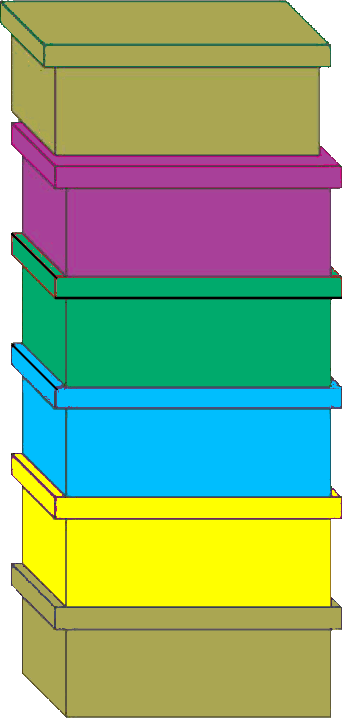
\includegraphics[width=0.75\textwidth]{stack-example-boxes}
  \caption{Boxes}%
  \label{fig:boxes}
\end{subfigure}
\hfill
\begin{subfigure}{0.25\textwidth}
  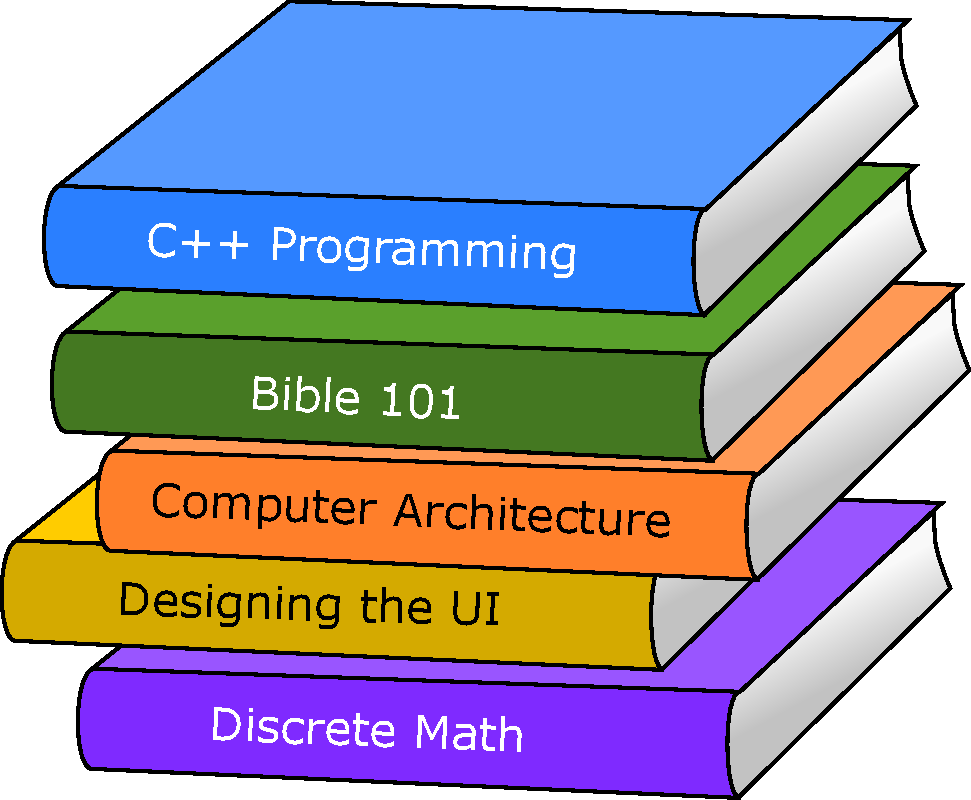
\includegraphics[width=\textwidth]{stack-example-books}
  \caption{Books}%
  \label{fig:books}
\end{subfigure}
%
% \caption{Creating subfigures in \LaTeX.}
\label{fig:figures}
\end{figure}
\end{frame}

\begin{frame}{Stack Example}
\begin{columns}[b]
  \column{0.66\textwidth}
    \onslide<1>{%
      \begin{tikzpicture}
        \Stack[A]{1}
      \end{tikzpicture}%
    }
    \hspace{5mm}
    \onslide<-2>{%
      \begin{tikzpicture}
        \Stack[B]{1}
      \end{tikzpicture}%
    }

    \onslide<-3>{%
      \hspace{1cm}\begin{tikzpicture}
        \Stack[C]{1}
      \end{tikzpicture}%
    }%
    \hspace{5mm}
    \onslide<-5>{%
      \begin{tikzpicture}
        \Stack[D]{1}
      \end{tikzpicture}%
    }

    \onslide<-6>{%
      \begin{tikzpicture}
        \Stack[E]{1}
      \end{tikzpicture}%
    }

  \column{0.33\textwidth}
    \centering
    \begin{tikzpicture}
      \only<1>{
        \node (stack) at (0,0)  [stack top, font=\tiny, align=center, name=stack]{};
        \node at (stack) [anchor=center, name=stack, align=left, yslant=0.5, xslant=-1, font=\footnotesize, text=black]{Empty\\Stack};
      }
      \only<2>{
        \Stack[A]{1}
        \node[above = of StackTop, align=center, anchor=center] {Push\\A};
      }
      \only<3>{
        \Stack[B]{2}
        \node[above = of StackTop, align=center, anchor=center] {Push\\B};
      }
      \only<4>{
        \Stack[C]{3}
        \node[above = of StackTop, align=center, anchor=center] {Push\\C};
      }
      \only<5>{
        \Stack[C]{3}
        \node[above = of StackTop, align=center, anchor=center] {Peek\\top};
      }
      \only<6>{
        \Stack[D]{4}
        \node[above = of StackTop, align=center, anchor=center] {Push\\D};
      }
      \only<7>{
        \Stack[E]{5}
        \node[above = of StackTop, align=center, anchor=center] {Push\\E};
      }
      \only<8>{
        \Stack[D]{4}
        \node[above = of StackTop, align=center, anchor=center] {Pop};
      }
      \only<9>{
        \Stack[C]{3}
        \node[above = of StackTop, align=center, anchor=center] {Pop};
      }
      
      % Reserve the space for the biggest stack size
      \invisible{\Stack{5}\node[above = of StackTop, align=center, anchor=center] {Push\\E};}
    \end{tikzpicture}
\end{columns}

\end{frame}

\begin{frame}{Stack Interface}
  \renewcommand{\umlfillcolor}{CSUblue!80!black}
  \renewcommand{\umldrawcolor}{white}
  \renewcommand{\umltextcolor}{white}
  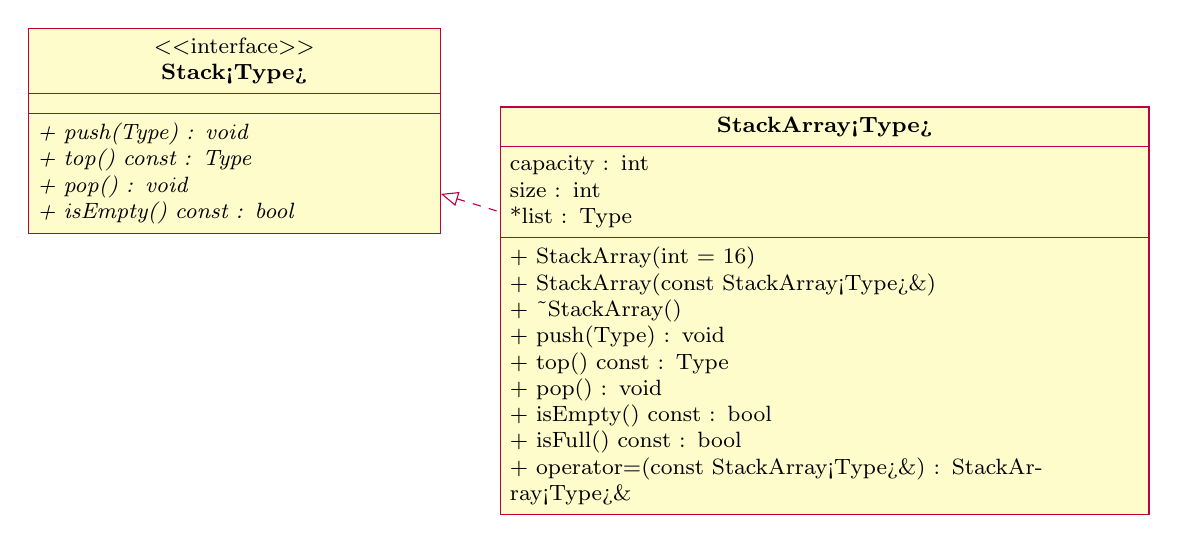
\begin{tikzpicture}[every node/.style={font=\footnotesize}]
    \begin{interface}{Stack<Type>}{0,0}
      \operation[0]{+ push(Type) : void}
      \operation[0]{+ top() const : Type}
      \operation[0]{+ pop() : void}
      \operation[0]{+ isEmpty() const : bool}
    \end{interface}

    \begin{class}[text width=8cm]{StackArray<Type>}{7.5,-1}
      \implement{Stack<Type>}
      \attribute{capacity : int}
      \attribute{size : int}
      \attribute{*list : Type}
      \operation{+ StackArray(int = 16)}
      \operation{+ StackArray(const StackArray<Type>\&)}
      \operation{+ \textasciitilde{}StackArray()}
      \operation{+ push(Type) : void}
      \operation{+ top() const : Type}
      \operation{+ pop() : void}
      \operation{+ isEmpty() const : bool}
      \operation{+ isFull() const : bool}
      \operation{+ operator=(const StackArray<Type>\&) : StackArray<Type>\&}
    \end{class}
  \end{tikzpicture}
\end{frame}

\section{Array Stack}
% \begin{frame}{Stack Operations}
% In the abstract Stack class, we may want the following operations
% \begin{itemize}
% \item
%   \lstinline{StackArray(const int capacity = 8)}
% \item
%   \lstinline{StackArray(const StackArray<Type>& src)}
% \item
%   \lstinline{isEmpty() const}
% \item
%   \lstinline{isFull() const}
% \item
%   \lstinline{push()}
% \item
%   \lstinline{top() const}
% \item
%   \lstinline{pop()}
% \item
%   ...
% \end{itemize}

% \end{frame}

\begin{frame}{Array-Based Stack Implementation}
\begin{itemize}
\item
  The first element goes in the first array position, the second in the second position, etc.
\item
  The top of the stack is an index of the last element added to the stack.
\item
  Stack elements may be stored in an array, which is a random-access data structure.
  \begin{itemize}
  \item
    The stack element is accessed only through the top.
  \end{itemize}
\item
  To track the top position, use a variable.
\end{itemize}

\end{frame}


\begin{frame}{Array-Based Stack Implementation}
\begin{itemize}
\item
  Can dynamically allocate an array.
\item
  Enables the user to specify the size of the array.
\end{itemize}
\end{frame}

\begin{frame}{Array-Based Stack Implementation}
\begin{itemize}
\item
  The \texttt{size} attribute will hold the number of elements currently in the array.
\item
  The top index is typically \texttt{size - 1} when \texttt{size} counts elements.
\item
  The \texttt{capacity} attribute will hold the maximum number of elements of the array before it needs to be resized.
\end{itemize}
\end{frame}

\begin{frame}{Array-Based Stack Implementation}
  \begin{tikzpicture}

    % Dynamic Array
    \ArrayLabel{}
    \ArrayNodeStack{A}
    \ArrayNodeStack{B}
    \ArrayNodeStack{C}
    \ArrayNodeStack{D}
    \onslide<2->{\ArrayGroupVerticleRight{elD}{elA}{Stack Elements}}
    \ArrayNodeStackSpan{}
    \ArrayNodeStack[CSUcyan][{[99]}]{}
    \onslide<3->{\ArrayGroupVerticleRight{prev}{space}{Unused}}

    % Stack Class Members
    \begin{scope}[node of array/.append style={minimum width=14mm}]
      \ArrayLabel[0][-3]{}
      \ArrayNodeStack[CSUgold][pList]{}
      \fill (prev) circle(3pt);
      \coordinate (ptrCircle) at (prev);
      \draw[link] (ptrCircle) to[bend right] (elA);

      \ArrayNodeStack[CSUcyan][size]{4}
      \ArrayNodeStack[CSUcyan][capacity]{100}
    \end{scope}
    \begin{scope}[on background layer]
      \node[draw,fill=CSUslate, very thick,fit=(el100) (el4) (el) (index)] (stackMembers) {};
    \end{scope}
    \node[anchor=south, font=\ttfamily] at ([yshift=0pt] stackMembers.north) {stack};
  \end{tikzpicture}
\end{frame}

\begin{frame}{Empty Array-Based Stack}
  \begin{tikzpicture}

    % Dynamic Array
    \ArrayLabel{}
    \ArrayNodeStack{A}
    \ArrayNodeStack{B}
    \ArrayNodeStack{C}
    \ArrayNodeStack{D}
    %\ArrayGroupVerticleRight{elD}{elA}{Stack Elements}
    \ArrayNodeStackSpan{}
    \ArrayNodeStack[CSUcyan][{[99]}]{}
    \ArrayGroupVerticleRight{prev}{elA}{Unused}

    % Stack Class Members
    \begin{scope}[node of array/.append style={minimum width=14mm}]
      \ArrayLabel[0][-3]{}
      \ArrayNodeStack[CSUgold][pList]{}
      \fill (prev) circle(3pt);
      \coordinate (ptrCircle) at (prev);
      \draw[link] (ptrCircle) to[bend right] (elA);

      \ArrayNodeStack[CSUcyan][size]{0}
      \ArrayNodeStack[CSUcyan][capacity]{100}
    \end{scope}
    \begin{scope}[on background layer]
      \node[draw,fill=CSUslate, very thick,fit=(el100) (el) (index)] (stackMembers) {};
    \end{scope}
    \node[anchor=south, font=\ttfamily] at ([yshift=0pt] stackMembers.north) {stack};
  \end{tikzpicture}
\end{frame}

\begin{frame}{Empty Array-Based Stack}
  \begin{tikzpicture}[stack instruction/.append style={fit={(stackMembers.east) (stackMembers.west)}, yshift=5em}]

    % Dynamic Array
    \ArrayLabel{}
    \alt<1>{
      \ArrayNodeStack{A}
    }{
      \ArrayNodeStack{u}
    }
    \alt<-3>{
      \ArrayNodeStack{B}
    }{
      \ArrayNodeStack{s}
    }
    \alt<-5>{
      \ArrayNodeStack{C}
    }{
      \ArrayNodeStack{c}
    }
    \ArrayNodeStack{D}
    %\ArrayGroupVerticleRight{elD}{elA}{Stack Elements}
    \ArrayNodeStackSpan{}
    \ArrayNodeStack[CSUcyan][{[99]}]{}

    \alt<1>{
      \ArrayGroupVerticleRight{prev}{elA}{Unused}
    }{
      \alt<-3>{
        \ArrayGroupVerticleRight{prev}{elB}{Unused}
      }{
        \alt<-5>{
          \ArrayGroupVerticleRight{prev}{elC}{Unused}
        }{
          \alt<-8>{
            \ArrayGroupVerticleRight{prev}{elD}{Unused}
          }{
            \ArrayGroupVerticleRight{prev}{elc}{Unused}
          }

        }
      }
    }

    \alt<1>{
    }{
      \alt<-3>{
        \ArrayGroupVerticleRight{elu}{elu}{Stack Elements}
      }{
        \alt<-5>{
          \ArrayGroupVerticleRight{els}{elu}{Stack Elements}
        }{
          \alt<-8>{
            \ArrayGroupVerticleRight{elc}{elu}{Stack Elements}
          }{
            \ArrayGroupVerticleRight{els}{elu}{Stack Elements}
          }

        }
      }
    }


    % Stack Class Members
    \begin{scope}[node of array/.append style={minimum width=14mm}]
      \ArrayLabel[0][-3]{}
      \ArrayNodeStack[CSUgold][pList]{}
      \fill (prev) circle(3pt);
      \coordinate (ptrCircle) at (prev);
      \draw[link] (ptrCircle) to[bend right] (elA);

      \alt<1>{
        \ArrayNodeStack[CSUcyan][size]{0}
      }{
        \alt<-3>{
          \ArrayNodeStack[CSUcyan][size]{1}
        }{
          \alt<-5>{
            \ArrayNodeStack[CSUcyan][size]{2}
          }{
            \alt<-8>{
              \ArrayNodeStack[CSUcyan][size]{3}
            }{
              \ArrayNodeStack[CSUcyan][size]{2}
            }
          }
        }
      }
      \ArrayNodeStack[CSUcyan][capacity]{100}
    \end{scope}
    \begin{scope}[on background layer]
      \node[draw,fill=CSUslate, very thick,fit=(el100) (el) (index)] (stackMembers) {};
    \end{scope}
    \node[anchor=south, font=\ttfamily] at ([yshift=0pt] stackMembers.north) {stack};

    % Task
    \alt<-2>{
      \node[stack instruction] at (stackMembers.north) {Push \lstinline{'u'}.};
    }{
      \alt<-4>{
        \node[stack instruction] at (stackMembers.north) {Push \lstinline{'s'}.};
      }{
        \alt<-6>{
          \node[stack instruction] at (stackMembers.north) {Push \lstinline{'c'}.};
        }{
          \alt<-7>{
            \node[stack instruction] at (stackMembers.north) {The top is \lstinline{'c'}.};
          }{
            \alt<-9>{
              \node[stack instruction] at (stackMembers.north) {Pop.};
            }{
              \node[stack instruction] at (stackMembers.north) {The top is \lstinline{'s'}.};
            }
          }
        }

      }
    }
    \onslide<10>{}
  \end{tikzpicture}
\end{frame}

\begin{frame}{Array-Based Stack Implementation}
  Resizing considerations
\begin{itemize}
\item
  If the array is fixed-size, pushing when \\\lstinline{size == capacity} causes overflow.
\item
  A common dynamic strategy is to allocate a new array with larger capacity
  (e.g., double the previous capacity) and copy elements. This gives
  \textit{amortized} \(O(1)\) time for \lstinline{push}.
\item
  Shrinking on pop is possible but should be done carefully to avoid
  frequent reallocations.
\end{itemize}
\end{frame}

\section{Linked Stack}


\begin{frame}{Linked Implementation of a Stack}
\begin{itemize}[<+->]\setlength\itemsep{0.5em}
\item
  Array only allows a fixed number of elements.
\item
  Must handle if pushed elements exceed the\\ array size.
\item
  Linked lists can dynamically organize data.
\item
  In a linked representation, \lstinline{mpHead} is a pointer to the memory address of the top element in the stack.\\
  (\lstinline{mpHead} may be named \lstinline{mpStackTop}.)
\end{itemize}
\end{frame}


\begin{frame}{Linked-List Implementation of a Stack}
  \begin{tikzpicture}[stack instruction/.append style={yshift=3em, anchor=north west}]

  \LinkPtr{mpStackTop}
  \only<7->{
    \LinkedNode{C}
  }
  \only<5->{
    \LinkedNode{B}
  }
  \onslide<3->{
    \LinkedNode{A}
  }

  \only<1>{
    \node[stack instruction] at (head.west) {Empty stack.};
  }
  
  \onslide<2->{
    \alt<-3>{
      \node[stack instruction] at (head.west) {Push \lstinline{'A'}.};
    }{
      \alt<-5>{
        \node[stack instruction] at (head.west) {Push \lstinline{'B'}.};
      }{
        \node[stack instruction] at (head.west) {Push \lstinline{'C'}.};
      }
    }
  }

  % Reserve space for this on a future slide
  \invisible{\LinkPtr[-2]{pNewNode}\LinkedNode{D}}
  \onslide<7>{}
  \end{tikzpicture}
\end{frame}

\begin{frame}{Push}
  \begin{tikzpicture}[stack instruction/.append style={yshift=3em, anchor=north west}]

  \LinkPtr{mpStackTop}
  \coordinate (mpStackTop) at (ptr);
  \alt<-3>{
    \LinkedNode{C}
  }{
    \LinkedNode[ptr][false]{C}
  }

  \LinkedNode{B}
  \LinkedNode{A}

  \node[stack instruction] at (head.west) {Push \lstinline{'D'}.};

  \onslide<2->{
    \LinkPtr[-2]{pNewNode}
    \LinkedNode{D}
    \onslide<4->{
      \draw[link] (mpStackTop) to [bend right=10] (elD);
    }
    \onslide<3->{
      \draw[link] (ptr) to [bend right=10] (elC);
    }
  }
  \end{tikzpicture}
\end{frame}

\begin{frame}{Pop}
  \begin{tikzpicture}[stack instruction/.append style={yshift=3em, anchor=north west}]

  \LinkPtr{mpStackTop}
  \coordinate (mpStackTop) at (ptr);
  \alt<-2>{
    \LinkedNode{D}
  }{
    \onslide<-3>{
      \LinkedNode[ptr][false]{D}
    }
  }
  \onslide<2->{
    \alt<-3>{
      \TailPtr{pToDelete}
    }{
      \TailPtr[null]{pToDelete}
    }
  }
  \alt<-3>{
    \LinkedNode{C}
  }{
    \LinkedNode[ptr][false]{C}
  }
  \LinkedNode{B}
  \LinkedNode{A}

  \onslide<3->{\draw[link] (mpStackTop) to [bend left] (elC);}

  \node[stack instruction] at (head.west) {Pop.};
  \onslide<4>{}

  % Reserve space for this on a future slide
  \invisible{\LinkPtr[-2]{pNewNode}\LinkedNode{D}}
  \end{tikzpicture}
\end{frame}


\begin{frame}{Linked Stack Performance}
\begin{itemize}[<+->]
\item
  \lstinline{push} and \lstinline{pop} are \(O(1)\) operations because they only change a set number of pointers.
\item
  Linked stacks do not require contiguous memory but have per-node overhead
  (pointer and allocation cost).
\end{itemize}
\end{frame}

\section{Postfix Notation}

\begin{frame}{Infix Notation}
\emph{Infix notation}: usual notation for writing arithmetic expressions
\begin{itemize}[<+->]
\item
  Operator is written between the operands.
\item
  Example: \(a + b\).
\item
  Evaluates from left to right.
\item
  Operators have precedence.
\item
  Parentheses can be used to override precedence.
\end{itemize}
\end{frame}

\begin{frame}{Prefix Notation (Polish Notation)}
\emph{Prefix (Polish) notation}: operators are written before the operands
\begin{itemize}
\item
  Introduced by the Polish mathematician Jan Lukasiewicz in the early 1920s.
\item
  Parentheses can be omitted.
\item
  Example: \(a + b\) becomes \(+\ a\ b\).
\end{itemize}
\end{frame}

\begin{frame}{Postfix Notation (Reverse Polish Notation)}
\emph{Postfix notation}: operators follow the operands (postfix operators)

\begin{itemize}
\item
  Proposed by Australian philosopher and early computer scientist, Charles L. Hamblin, in the late 1950s.
\item
  Advantage: operators appear in the order required for computation.
\item
  Example: \(a + b\) becomes \(a\ b\ + \).
\item
  Example: \(a + b \cdot c\) becomes \(a\ b\ c\ \cdot\ + \)
\item
  Example: \((a + b) \cdot c\) becomes \(a\ b + c\ \cdot \)
\end{itemize}
\end{frame}

\begin{frame}{Postfix Notation Examples}
\center{%
\begin{tabular}{l l}
\toprule
  \textbf{Infix Expression} & \textbf{Equivalent Postfix Express} \\
\midrule
  \(a + b\) & \(a\ b\ + \) \\
  \(a + b \cdot c\) & \(a\ b\ c \cdot + \) \\
  \(a \cdot b + c\) & \(a\ b \cdot c\ + \) \\
  \((a + b) \cdot c\) & \(a\ b + c\ \cdot \) \\
  \((a - b) \cdot (c + d)\) & \(a\ b - c\ d\ +\ \cdot \) \\
  \((a + b) \cdot (c - d / e)\) & \(a\ b + c\ d\ e\ /\ -\ \cdot \) \\
  \((a + b) \cdot (c - d / e) + f\) & \(a\ b + c\ d\ e\ /\ -\ \cdot\ f\ + \) \\
\bottomrule
\end{tabular}%
}
\end{frame}

\begin{frame}{Postfix Notation Example}
\center{%
\begin{align*}
    & (1 + 7) \cdot (6 - 12 / 3)\\
    \\
    & 1\ \ 7 + 6\ \ 12\ \ 3\ /\ -\ \cdot \\
  =\ & 8\ \ 6\ \ 12\ \ 3\ /\ -\ \cdot \\
  =\ & 8\ \ 6\ \ 4\ -\ \cdot \\
  =\ & 8\ \ 2\ \cdot \\
  =\ & 16
\end{align*}
}
\end{frame}

\begin{frame}{Postfix Expressions Calculator}
Postfix notation has important applications in\\ computer science.

Many compilers first translate arithmetic expressions\\ into postfix notation and then translate this expression\\ into machine code.

Evaluation algorithm:\vspace{-0.5em}
\begin{itemize}
  \item
    Scan expression from left to right.
  \item
    When an operator is found, back up to get operands, perform the operation, and continue.
\end{itemize}
\end{frame}

\begin{frame}{Postfix Expressions Calculator}
Expression: \(6\ 3 + 2\ *\ =\)


\begin{columns}
\column{0.6\textwidth}
  \alt<-2>{%
    Push \lstinline{6} onto the stack.
  }{%
    \alt<-4>{%
      Push \lstinline{3} onto the stack.
    }{%
      \alt<-7>{%
        \lstinline{+}\\
        Pop stack twice.\\
        op2 = 3;\\
        op1 = 6;
      }{%
        \alt<-9>{
          \lstinline{op1 + op2 = 9}\\
          Push \lstinline{9} onto the stack.
        }{
          \alt<-11>{
            Push \lstinline{2} onto the stack.
          }{
            \alt<-16>{
              \lstinline{*}\\
              Pop stack twice.\\
              op2 = 2;\\
              op1 = 9;
            }{
              \alt<-18>{
                \lstinline{op1 * op2 = 18}\\
                Push \lstinline{18} onto the stack.
              }{
                \lstinline{=}\\
                Pop stack and print: \lstinline{18}\\
              }

            }

          }
        }
      }
    }
  }

\column{0.3\textwidth}
  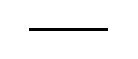
\begin{tikzpicture}[span of array/.append style={minimum height=8mm,}, stack instruction/.append style={anchor=south}]
    % Line representing the empty stack.
    \draw[very thick] (-5mm, 0.36) to (5mm, 0.36);
    \ArrayLabel{Stack}
    \alt<-7>{
      \onslide<2-6>{
        \ArrayNodeStackSpan[6]{}
      }

      \onslide<4-5>{
        \ArrayNodeStackSpan[3]{}
      }
    }{
      \alt<-17>{
        \onslide<9-13>{\ArrayNodeStackSpan[9]{}}
        \onslide<11-12>{\ArrayNodeStackSpan[2]{}}
      }{
        \onslide<18-19>{\ArrayNodeStackSpan[18]{}}
        \onslide<1>{\ArrayNodeStackSpan[]{}} % Never displayed but holds space.
      }
    }

  \onslide<20>{}
  \end{tikzpicture}
\end{columns}
\end{frame}

\begin{frame}{Postfix Expressions Calculator}
Symbols can be numbers or anything else:
\begin{itemize}
  \item
    \(+\), \(-\), \(*\), and \(/\) are operators, require two operands.
  \begin{itemize}
    \item
      Pop stack twice and evaluate the expression.
    \item
      If the stack has less than two elements, then error.
  \end{itemize}
  \item
    If the symbol is \(=\), the expression ends.
    \begin{itemize}
      \item
        Pop and print the answer from the stack.
      \item
        If the stack has more than one element, then error.
    \end{itemize}
  \item
    If the symbol is anything undefined, the expression contains an illegal operator.
\end{itemize}
\end{frame}

\begin{frame}[fragile]{Postfix Expressions Calculator}
Start to the function:
\begin{lstlisting}
bool evaluatePostfixExpression(ifstream &input, double& result)
{
  Stack<double> stack;
  char nextSymbol;
  double value;

  // ...
  nextSymbol = input.peek();
  // ...
}
\end{lstlisting}
\end{frame}

\begin{frame}{Postfix Expressions Calculator}
Notes on error handling
\begin{itemize}
  \item
    Decide whether the API throws exceptions on underflow/overflow or returns
  error codes. Be consistent across the codebase.
  \item
    For numeric evaluation, consider handling divide-by-zero and invalid tokens.
\end{itemize}
\end{frame}

% \begin{frame}{Postfix Expressions Calculator}
% Assume postfix expressions are in this form:\\
% \texttt{\#6 \#3 + \#2 * =}
% \begin{itemize}
%   \item
%     If symbol scanned is \#, next input is a number
%   \item
%     If the symbol scanned is not \#, then it is:
%     \begin{itemize}
%       \item
%         An operator (may be illegal) or
%       \item
%         An equal sign (end of expression)
%     \end{itemize}
%   \item
%     Assume the expressions contain only \(+\), \(-\), \(*\), and \(/\) operators.
% \end{itemize}
% \end{frame}

% \begin{frame}[fragile]{Postfix Expressions Calculator}
% Pseudocode:\\
% \begin{lstlisting}
% Read the first character
% while not the end of the input data
% {
%   a. initialize the stack
%   b. process the expression
%   c. output the result
%   g. get the next expressions
% }
% \end{lstlisting}
% \end{frame}

\section{SLList in Reverse}

\begin{frame}{Iterating Over a Linked List in Reverse}
\begin{itemize}
  \item
    To print a list backward non-recursively, first get\\ to the last node of the list.
    \begin{itemize}
      \item
        Problem: Links go in only one direction.
      \item
        Solution: Save a pointer to each node in a stack.\\
        Uses the LIFO principle.
    \end{itemize}
  \item
    Since the number of nodes is usually not known, use the linked implementation of a stack.
\end{itemize}  
\end{frame}

\begin{frame}{Iterating Over a Linked List in Reverse}
  \centering
  \onslide<-8>{
    While \lstinline{pCurrent} is not null, push it on the stack and go to next.
  }
  \onslide<9->{
    While the stack is not empty, access the top and pop.
  }

  \begin{tikzpicture}[span of array/.append style={minimum height=6mm, minimum width=6mm}, stack instruction/.append style={anchor=south}, node of array/.append style = {fill=CSUgold}]
    \LinkPtr{pHead}
    \LinkedNode{5}
    \onslide<2-3>{\TailPtr{pCurrent}}
    \onslide<14-15>{\TailPtr{pCurrent}}
    \LinkedNode{10}
    \onslide<4-5>{\TailPtr{pCurrent}}
    \onslide<12-13>{\TailPtr{pCurrent}}
    \LinkedNode{15}
    \onslide<6-11>{
      \alt<8-9>{
        \TailPtr[null]{pCurrent}
      }{
        \TailPtr{pCurrent}
      }
    }

    % Line representing the empty stack.
    \draw[very thick] (-4cm - 3mm, -0.64) to (-4cm + 3mm, -0.64);
    
    \ArrayLabel[-1][-4]{Stack}
    \onslide<3-14>{
      \ArrayNodeStackSpan[]{}
      %\node[pointer, name=ptr2] at (prev) {};
      \fill (prev) circle(2pt);
      \coordinate (ptr) at (prev);
      \draw[link, ->] (ptr) to[bend left] (el5);
    }
    \onslide<5-12>{
      \ArrayNodeStackSpan[]{}
      %\node[pointer, name=ptr2] at (prev) {};
      \fill (prev) circle(2pt);
      \coordinate (ptr) at (prev);
      \draw[link, ->] (ptr) to[bend left] (el10);
    }
    \onslide<7-10>{
      \ArrayNodeStackSpan[]{}
      %\node[pointer, name=ptr2] at (prev) {};
      \fill (prev) circle(2pt);
      \coordinate (ptr) at (prev);
      \draw[link, ->] (ptr) to[bend left] (el15);
    }
    \onslide<15>{}
  \end{tikzpicture}
\end{frame}

\section{Review}

\begin{frame}{Summary}
\emph{Stack}: items are added/deleted from one end.
\begin{itemize}
  \item
    Last-In, First-Out (LIFO) data structure
  \item
    Operations: push, pop, peek/pop, initialize, destroy, \lstinline{isEmpty}, \lstinline{isFull} (for fixed size)
  \item
    Can be implemented as an array or linked list.
  \item
    Middle elements should not be accessed directly.
\end{itemize}
\end{frame}


\begin{frame}{Space and Performance}
\begin{itemize}
  \item 
    \lstinline{push}, \lstinline{pop}, and \lstinline{peek} are \(O(1)\) time\\ (if not resizing an array).
  \item 
    \textit{Array stacks} use contiguous memory and\\ have
  lower per-element overhead.\\
  \textit{Linked stacks} use extra memory per node but
  grow without large reallocations.
  \item 
    \emph{Postfix notation}: operators are written after the operands; this
  form is convenient for stack-based evaluation and for compiler internals.
\end{itemize}
\end{frame}

\end{document}
